%%%%%%%%%% Prefix a "S" to all equations, figures, tables and reset the counter %%%%%%%%%%
\setcounter{equation}{0}
\setcounter{figure}{0}
\setcounter{table}{0}
\setcounter{page}{1}
\makeatletter
%\renewcommand{\theequation}{S\arabic{equation}}
\renewcommand{\thefigure}{S\arabic{figure}}
%\renewcommand{\bibnumfmt}[1]{[S#1]}
%\renewcommand{\citenumfont}[1]{S#1}
%%%%%%%%%%%%%%%%%%%%

\section{Supplementary Figures}
\begin{figure}[hbt!]
    \centering
        \sidesubfloat[]{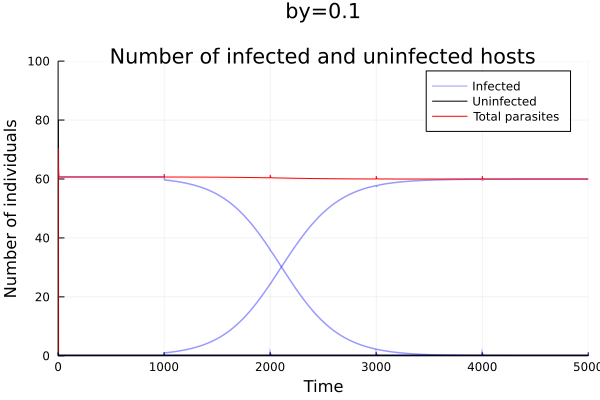
\includegraphics[width=0.4\textwidth]{figures/supp_1a.png}\label{fig:a}}
    \hfil
        \sidesubfloat[]{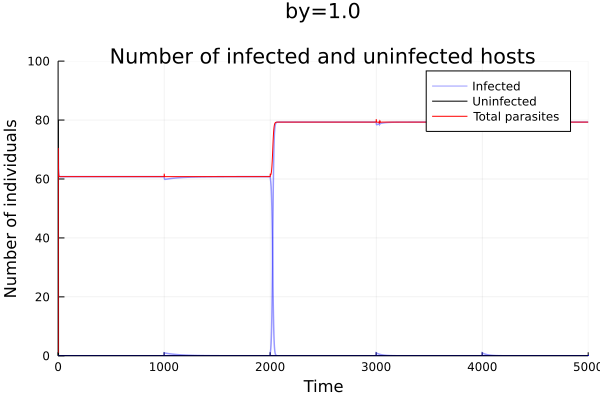
\includegraphics[width=0.4\textwidth]{figures/supp_1b.png}\label{fig:b}}

    \medskip
        \sidesubfloat[]{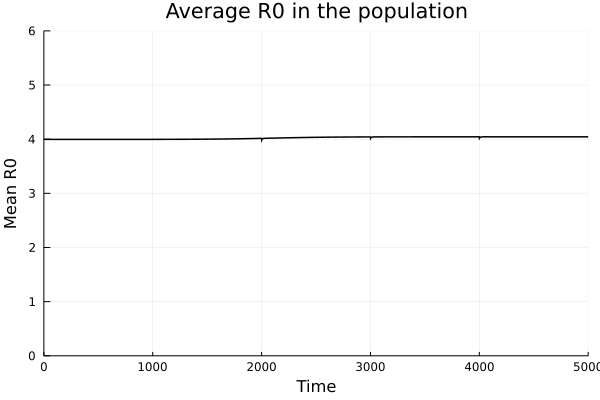
\includegraphics[width=0.4\textwidth]{figures/supp_1c.png}\label{fig:c}}
    \hfil
        \sidesubfloat[]{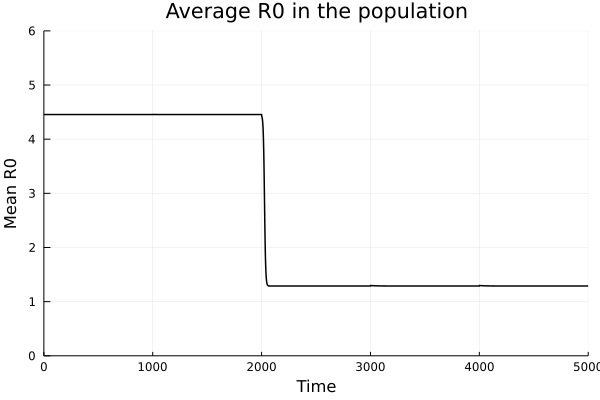
\includegraphics[width=0.4\textwidth]{figures/supp_1d.png}\label{fig:d}}

    \medskip
        \sidesubfloat[]{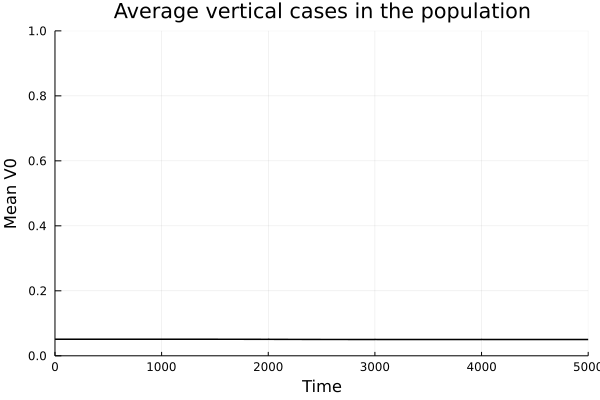
\includegraphics[width=0.4\textwidth]{figures/supp_1e.png}\label{fig:e}}
    \hfil
        \sidesubfloat[]{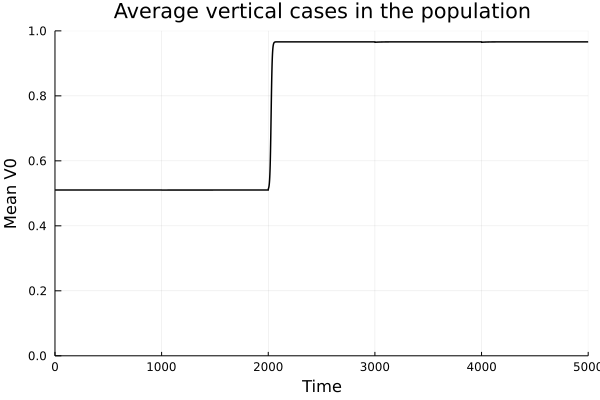
\includegraphics[width=0.4\textwidth]{figures/supp_1f.png}\label{fig:f}}

    \medskip
        \sidesubfloat[]{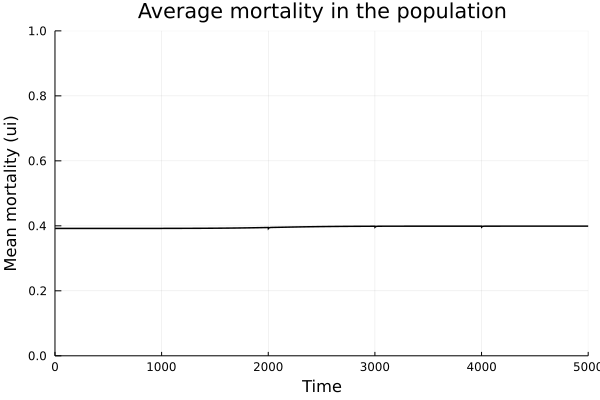
\includegraphics[width=0.4\textwidth]{figures/supp_1g.png}\label{fig:g}}
    \hfil
        \sidesubfloat[]{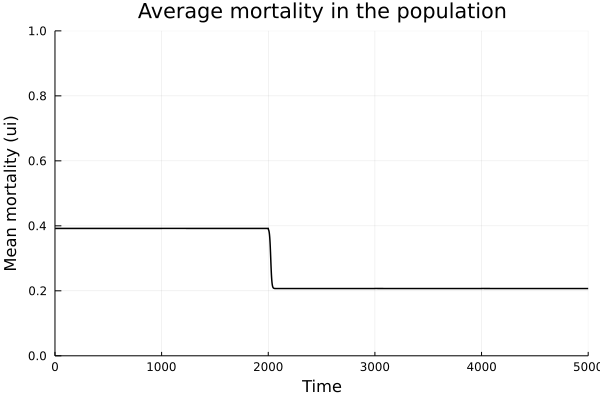
\includegraphics[width=0.4\textwidth]{figures/supp_1h.png}\label{fig:h}}
        
    \medskip
        \sidesubfloat[]{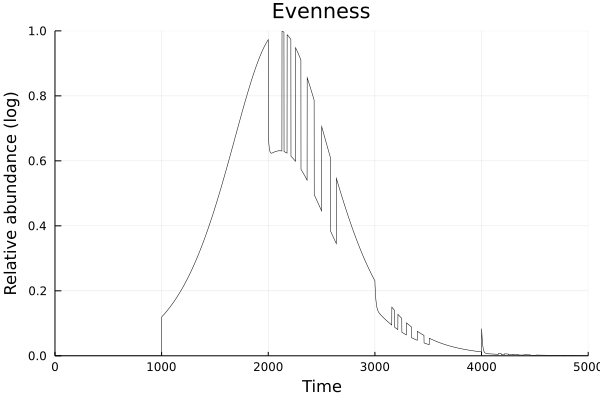
\includegraphics[width=0.4\textwidth]{figures/supp_1i.png}\label{fig:i}}
    \hfil
        \sidesubfloat[]{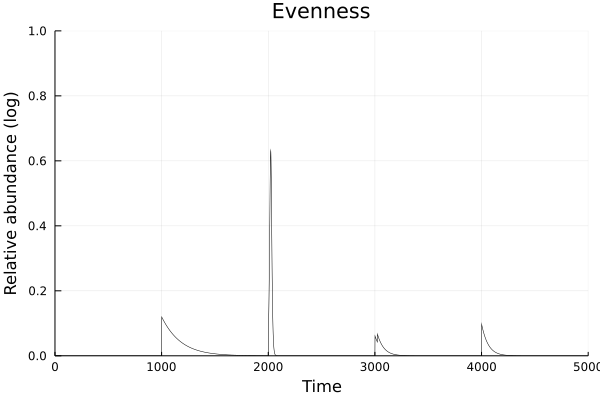
\includegraphics[width=0.4\textwidth]{figures/supp_1j.png}\label{fig:j}}
\caption{\textbf{Evolutionary dynamics of 100 infected strains introduced every 1,000 generations for two vertical transmission values, $b_i = 0.1$ (left column) and $b_i = 1.0$ (right column)}. We demonstrate (a,b) the number of uninfected and infected hosts with each strain; (c,d) the mean $R_0$ in the population; (e,f) the average of all new infections acquired vertically; (g,h) the average mortality in the population; (i,j) the evenness of the total population for 5,000 time-steps.
}
    \label{fig:SF1}
\end{figure}

\begin{figure}[tbp]
    \centering
        \sidesubfloat[]{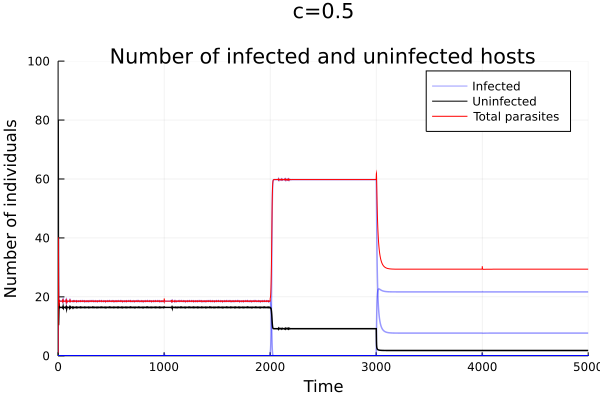
\includegraphics[width=0.4\textwidth]{figures/supp_2a.png}\label{fig:a}}
    \hfil
        \sidesubfloat[]{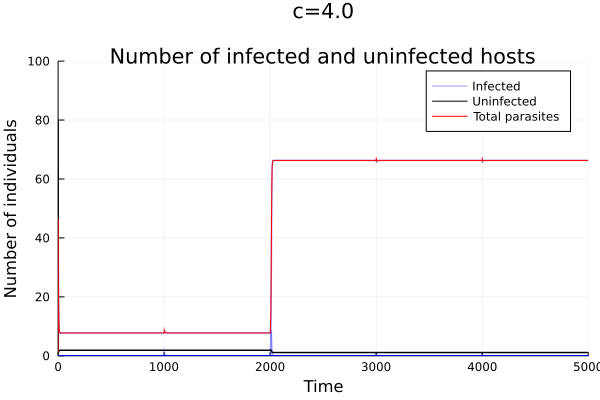
\includegraphics[width=0.4\textwidth]{figures/supp_2b.png}\label{fig:b}}

    \medskip
        \sidesubfloat[]{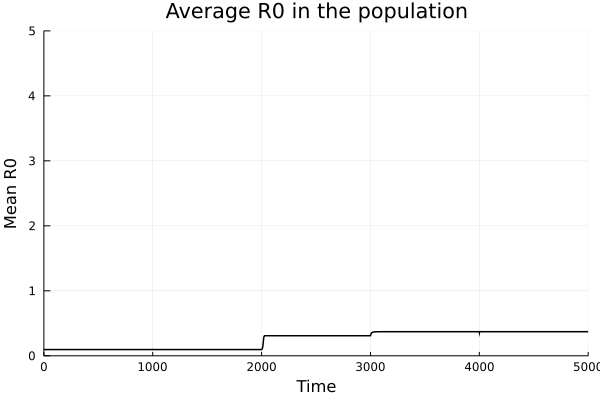
\includegraphics[width=0.4\textwidth]{figures/supp_2c.png}\label{fig:c}}
    \hfil
        \sidesubfloat[]{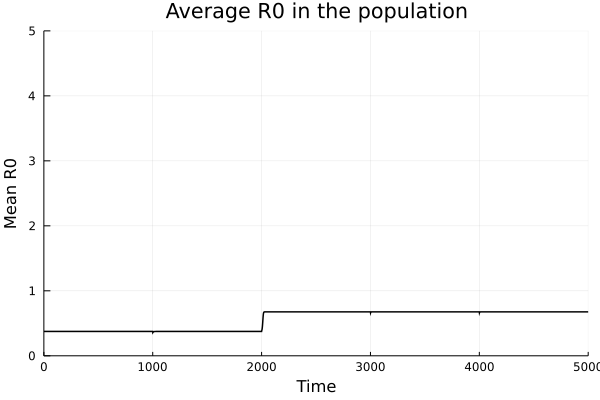
\includegraphics[width=0.4\textwidth]{figures/supp_2d.png}\label{fig:d}}

    \medskip
        \sidesubfloat[]{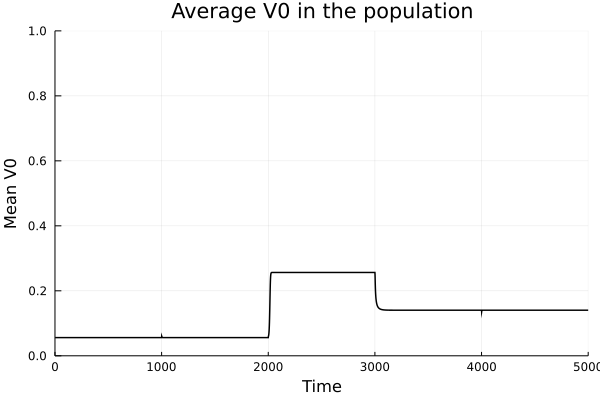
\includegraphics[width=0.4\textwidth]{figures/supp_2e.png}\label{fig:e}}
    \hfil
        \sidesubfloat[]{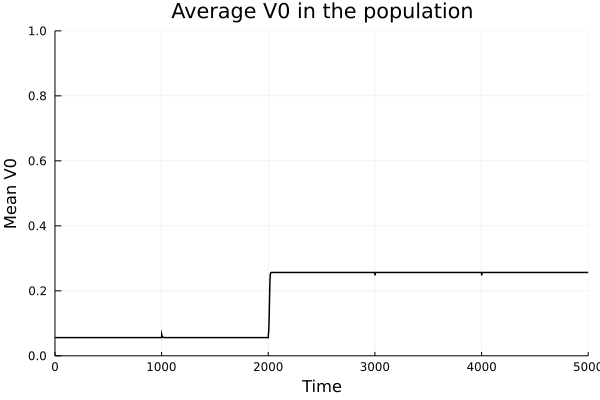
\includegraphics[width=0.4\textwidth]{figures/supp_2f.png}\label{fig:f}}

    \medskip
        \sidesubfloat[]{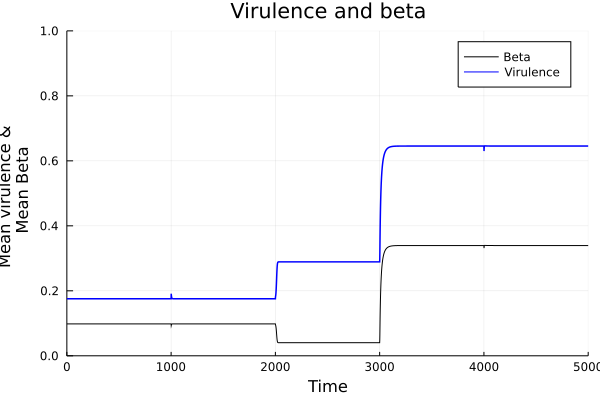
\includegraphics[width=0.4\textwidth]{figures/supp_2g.png}\label{fig:g}}
    \hfil
        \sidesubfloat[]{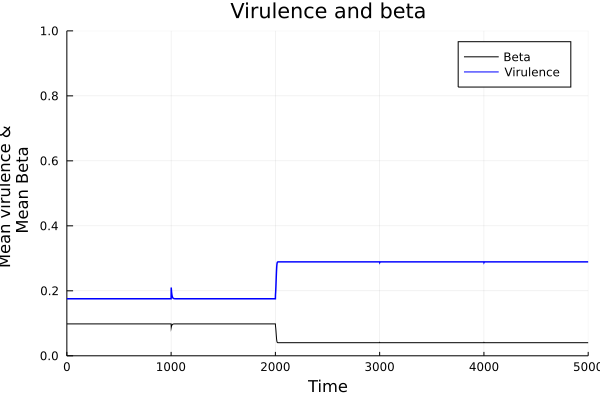
\includegraphics[width=0.4\textwidth]{figures/supp_2h.png}\label{fig:h}}
        
    \medskip
        \sidesubfloat[]{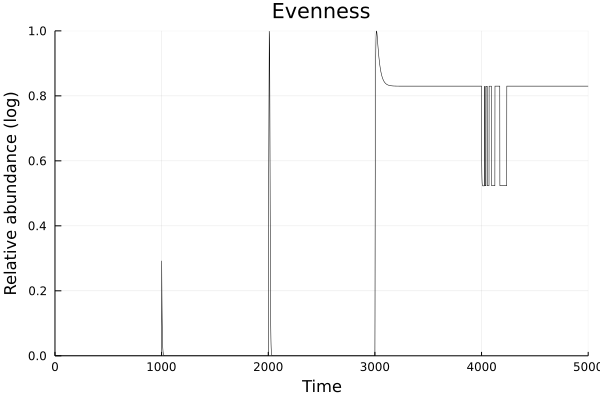
\includegraphics[width=0.4\textwidth]{figures/supp_2i.png}\label{fig:i}}
    \hfil
        \sidesubfloat[]{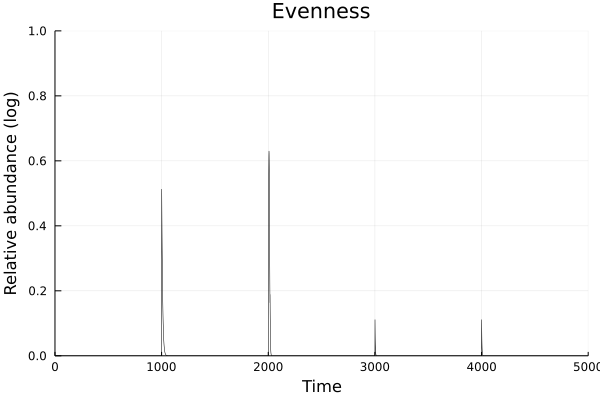
\includegraphics[width=0.4\textwidth]{figures/supp_2j.png}\label{fig:j}}
\caption{\textbf{Evolutionary dynamics of 100 infected strains introduced every 1,000 generations for two horizontal transmission opportunity, $c = 0.5$ (left column) and $c = 4.0$ (right column).} The parameters are identical to those in Figure 1 but with $e_i$, $b_i$ and $\beta_i$ constrained through equations (\ref{eqn:9}), (\ref{eqn:10}) and (\ref{eqn:11}). We demonstrate (a,b) the number of uninfected and infected hosts with each strain; (c,d) the mean $R_0$ in the population; (e,f) the average of all new infections acquired vertically; (g,h) the average virulence and horizontal transmission rate $\beta_i$; (i,j) the evenness of the total population for 5000 time-steps.
}
    \label{fig:SF2}
\end{figure}

\begin{figure}[tbp]
    \centering
        \sidesubfloat[]{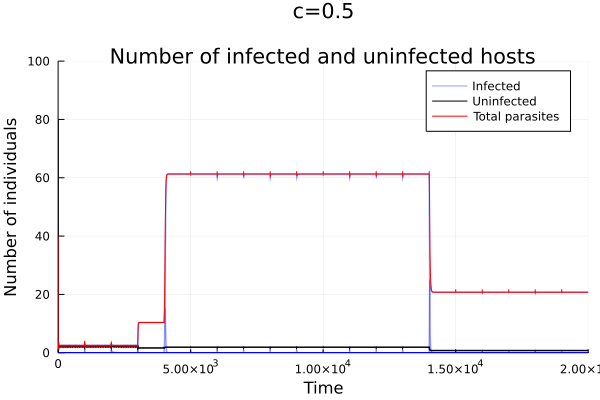
\includegraphics[width=0.4\textwidth]{figures/supp_3a.png}\label{fig:a}}
    \hfil
        \sidesubfloat[]{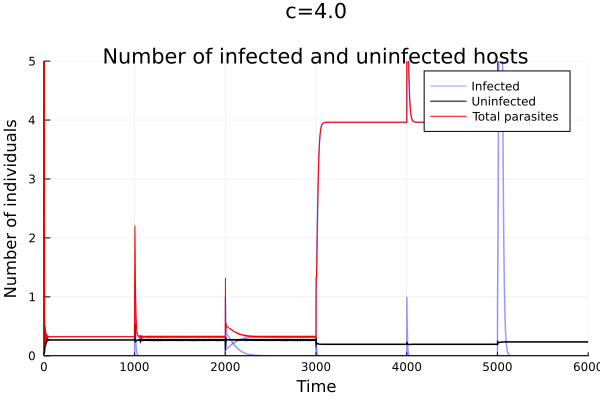
\includegraphics[width=0.4\textwidth]{figures/supp_3b.png}\label{fig:b}}

    \medskip
        \sidesubfloat[]{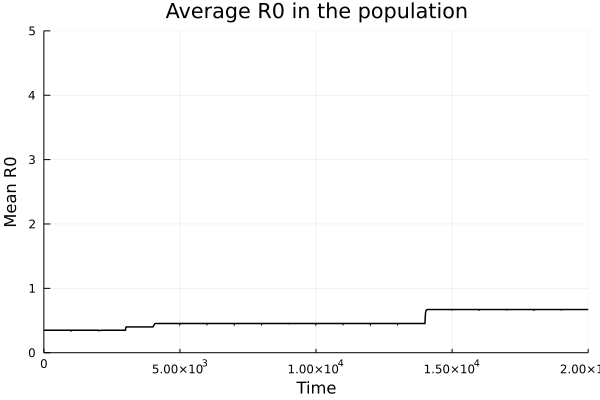
\includegraphics[width=0.4\textwidth]{figures/supp_3c.png}\label{fig:c}}
    \hfil
        \sidesubfloat[]{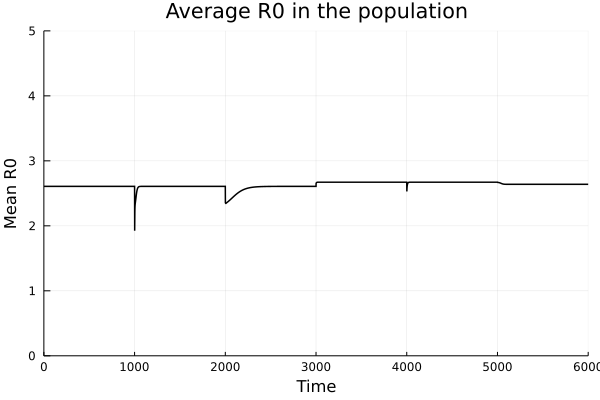
\includegraphics[width=0.4\textwidth]{figures/supp_3d.png}\label{fig:d}}

    \medskip
        \sidesubfloat[]{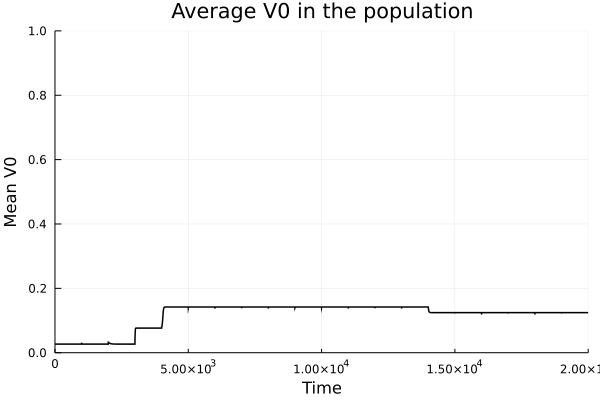
\includegraphics[width=0.4\textwidth]{figures/supp_3e.png}\label{fig:e}}
    \hfil
        \sidesubfloat[]{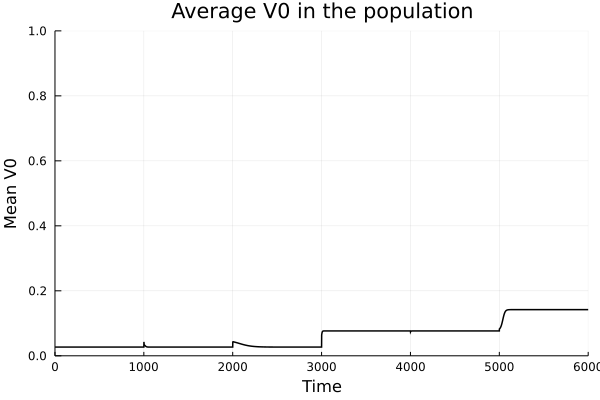
\includegraphics[width=0.4\textwidth]{figures/supp_3f.png}\label{fig:f}}

    \medskip
        \sidesubfloat[]{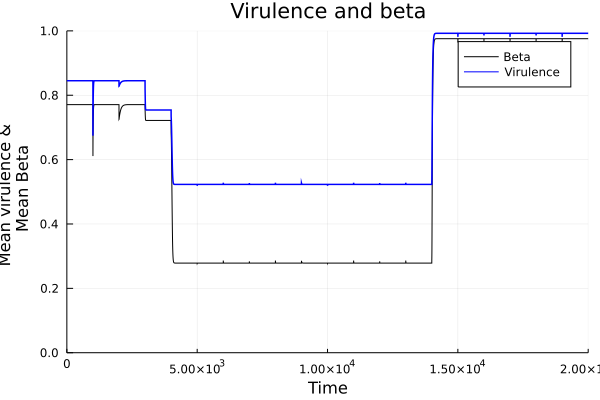
\includegraphics[width=0.4\textwidth]{figures/supp_3g.png}\label{fig:g}}
    \hfil
        \sidesubfloat[]{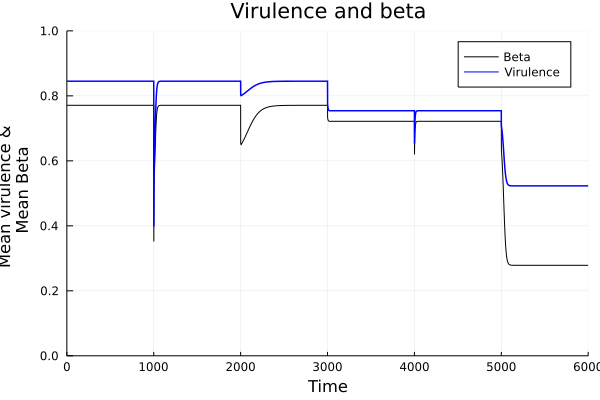
\includegraphics[width=0.4\textwidth]{figures/supp_3h.png}\label{fig:h}}
        
    \medskip
        \sidesubfloat[]{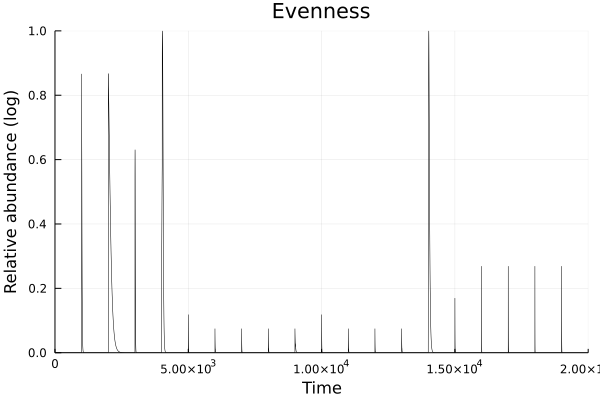
\includegraphics[width=0.4\textwidth]{figures/supp_3i.png}\label{fig:i}}
    \hfil
        \sidesubfloat[]{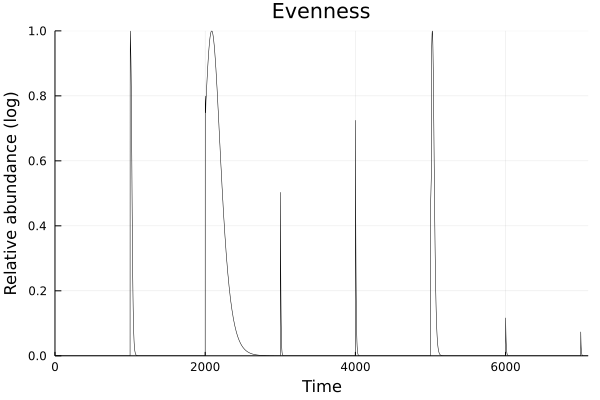
\includegraphics[width=0.4\textwidth]{figures/supp_3j.png}\label{fig:j}}
\caption{\textbf{Evolutionary dynamics of 100 infected strains introduced every 1,000 generations for two values of horizontal transmission opportunity values, $c = 0.5$ (left column) and $c = 4.0$ (right column).} All parameters are identical to those in Figure 2 but with a constraint $r_3$ value chosen randomly from a uniform distribution over [0, $r_1$] per strain. We demonstrate (a,b) the number of uninfected and infected hosts with each strain; (c,d) the mean $R_0$ in the population; (e,f) the average of all new infections acquired vertically; (g,h) the average virulence and horizontal transmissibility $\beta_i$; (i,j) the evenness of the total population for 20,000 and 6,000 time-steps for left and right column, respectively.
}
    \label{fig:SF3}
\end{figure}